% Provenance (never printed): cycle 4 SVT, "La planete Terre, l'environnement
% et l'action humaine": resources from the Earth, their geological origin, the
% time they take to form and the rate we use them; see
% sources/book1/PROVENANCE.md. Book 1, grade 9, chapter 3.
% Vocabulary guard: owns ore deposit (with concentration factor), aggregate,
% reserve. Resource, renewable resource, ore, raw material (chemistry grade
% 5), fossil fuels (chemistry grade 8) and element abundances (chemistry
% grade 9) are recalled in prose. Groundwater and aquifers are g6's. Coal,
% oil and gas are told, not defined: "source rock", "reservoir", "seal",
% "trap" and the coal ranks belong to Book 2 g11 (fossil-fuel-geology);
% "hydrothermal" is not used (later books). Scientific notation (grade 9).
\chapter{Grondstoffen uit de Aarde}\label{ch:g9:earth-resources}

Een smartphone past in een broekzak, maar bevat tientallen chemische
elementen: koper voor de draden, neodymium voor de magneten van de
luidspreker, gallium voor het licht van het scherm, indium voor de dunne
laag op het scherm die elektriciteit geleidt, en nog veel meer. Elk ervan
is ergens op de Aarde uit de grond gehaald. Een huis bevat veel meer: een
gemiddeld eengezinshuis heeft ongeveer honderd ton \omterm{def:g3:stones-pebbles-sand:sand}{zand}, \omterm{def:g3:stones-pebbles-sand:pebble}{grind} en
steenslag nodig, en zijn aandeel in de straten en scholen eromheen
ongeveer drie keer zoveel. Waar in de Aarde worden deze materialen
gevonden, en waarom juist daar?
% ledger: usgs:smartphone, usgs:aggregate (114 and 328 short tons: about 100 and 300 t)

\begin{recall}
In de scheikunde leer je dat de materialen die we uit de natuur halen
\emph{grondstoffen} zijn; een \emph{erts} is een \omterm{def:g3:stones-pebbles-sand:rock}{gesteente} waaruit een
metaal kan worden gewonnen; een \emph{hernieuwbare} grondstof wordt door de
natuur even snel aangevuld als we haar gebruiken; steenkool, aardolie en
aardgas zijn \emph{fossiele brandstoffen}; en zuurstof, silicium,
aluminium en ijzer zijn de meest voorkomende elementen van de korst.
\omterm{def:g6:water-underground:groundwater}{Grondwater} vult de \omterm{def:g6:water-underground:porosity}{poriën} van een \omterm{def:g6:water-underground:aquifer}{watervoerende laag}, en \omterm{def:g4:clouds-rain-snow:precipitation}{regen} vult die
weer aan (\cref{ch:g6:water-underground}). \omterm{def:g7:sediments-and-fossils:sediment}{Sedimenten} stapelen zich op in
lagen en worden sedimentgesteenten (\cref{ch:g7:sediments-and-fossils}),
in tijden die in miljoenen jaren worden geteld
(\cref{ch:g7:geological-time}).
\end{recall}

\section{Waarom een metaal geconcentreerd moet zijn}

Koper is overal: een gewoon \omterm{def:g3:stones-pebbles-sand:rock}{gesteente} bevat er een beetje van, een paar
gram per honderd kilogram. Maar om één kilogram koper uit zo'n \omterm{def:g3:stones-pebbles-sand:rock}{gesteente} te
halen, zou je er tonnen van moeten afgraven, vermalen en behandelen.
Mijnbouw loont alleen waar de natuur het metaal heeft verzameld in een veel
rijker \omterm{def:g3:stones-pebbles-sand:rock}{gesteente}.
% ledger: perkins:ore-grades (copper 0.006 % of the crust)

\begin{definition}[Ertsafzetting en concentratiefactor]\label{def:g9:earth-resources:ore-deposit}
Een \emph{ertsafzetting}\index{ertsafzetting} is een gesteentemassa waarin
natuurlijke processen een metaal of een \omterm{def:g6:rocks-and-minerals:mineral}{mineraal} genoeg hebben
geconcentreerd om het met winst te kunnen winnen. De
\emph{concentratiefactor}\index{concentratiefactor} van een metaal is het
aantal keer dat zijn gehalte in het erts groter is dan zijn gemiddelde
gehalte in de korst:
\[
\text{concentratiefactor} = \frac{\text{gehalte in het erts}}{\text{gemiddeld gehalte in de korst}} .
\]
\end{definition}
% ledger: perkins:ore-grades, earle:ore-grades

De gewone metalen van de korst, aluminium en ijzer, hoeven maar ongeveer
vier keer te worden geconcentreerd. Koper heeft ongeveer 80 keer nodig,
zink ongeveer 600 keer, en de zeldzaamste metalen van de grafiek, goud,
tin en chroom, duizenden keren. Hoe zeldzamer een metaal in de korst, hoe
meer de natuur moet doen om er een erts van te maken, en hoe minder
plaatsen waar ze dat heeft gedaan.
% ledger: perkins:ore-grades, earle:ore-grades

\begin{example}[Koper]
De korst bevat gemiddeld \qty{0.006}{\%} koper; een kopererts kan vanaf
ongeveer \qty{0.5}{\%} worden gewonnen. De \omterm{def:g9:earth-resources:ore-deposit}{concentratiefactor} is $0.5 \div 0.006
\approx 83$, ongeveer 80, of dicht bij $10^2$. Een ander leerboek neemt
\qty{40}{ppm} (\qty{0.004}{\%}) voor gewoon \omterm{def:g3:stones-pebbles-sand:rock}{gesteente} en \qty{1}{\%} voor
het erts: $1 \div
0.004 = 250$. De twee getallen verschillen, maar ze zeggen allebei
hetzelfde: een kopererts is ongeveer honderd keer rijker dan gewoon
\omterm{def:g3:stones-pebbles-sand:rock}{gesteente}.
\end{example}
% ledger: perkins:ore-grades, earle:ore-grades

\begin{omfigure}
\begin{tikzpicture}
\begin{axis}[xbar, xmode=log, width=12cm, height=5.3cm, xmin=1, xmax=2e4,
  log origin=infty, bar width=9pt, enlarge y limits=0.1,
  ytick=data, yticklabels={aluminium, ijzer, koper, zink, goud, tin, chroom},
  y dir=reverse, xlabel={concentratiefactor (logaritmische schaal)},
  xtick={1,10,100,1000,10000}, xticklabels={$1$,$10$,$10^2$,$10^3$,$10^4$},
  tick label style={font=\footnotesize}, label style={font=\small},
  nodes near coords, nodes near coords style={font=\scriptsize, anchor=west},
  point meta=explicit, xmajorgrids, grid style={black!12}]
\addplot[fill=omWarm!45, draw=omWarm!80!black] table[x=factor, y=x, meta=factor] {figdata/out/grade-9-concentration.dat};
\end{axis}
\end{tikzpicture}

{\small Hoeveel keer de natuur zeven metalen moet concentreren om een
winbaar erts te maken: het minimale gehalte van het erts gedeeld door het
gemiddelde gehalte van de korst. Elke stap van de schaal is tien keer de
vorige. Gegevens: D.~Perkins en anderen, \emph{Mineralogy}, en, voor goud,
S.~Earle, \emph{Environmental Geology}.}
% ledger: perkins:ore-grades, earle:ore-grades (figdata/grade-9/concentration.py)
\label{fig:g9:earth-resources:factors}
\end{omfigure}

\begin{method}[Een concentratiefactor berekenen]
\begin{enumerate}
  \item Schrijf het gehalte van het metaal in het erts en in de gemiddelde
        korst in dezelfde eenheid (procent, of gram per ton).
  \item Deel het gehalte in het erts door het gehalte in de korst.
  \item Rond het resultaat af: het gaat om de grootte, ongeveer 10, 100 of
        1000, die je als macht van tien kunt schrijven.
\end{enumerate}
\end{method}


\section{Hoe ertsafzettingen ontstaan}

De natuur concentreert metalen op verscheidene manieren. Drie ervan staan hieronder.

\begin{omfigure}
\begin{tikzpicture}[x=1cm, y=1cm, font=\footnotesize, >={Stealth[length=2mm]}]
  % country rock
  \fill[black!13] (0,0) rectangle (13,4.6);
  % surface with a valley on the right
  \fill[white] (0,4.6) -- (8.4,4.6) -- (9.6,3.7) -- (11.2,3.7) -- (12.0,4.6) -- (13,4.6) -- (13,5.6) -- (0,5.6) -- cycle;
  \draw[black!60] (0,4.6) -- (8.4,4.6) -- (9.6,3.7) -- (11.2,3.7) -- (12.0,4.6) -- (13,4.6);
  % river gravels on the valley floor
  \fill[omLithCongl] (9.5,3.75) -- (11.3,3.75) -- (11.15,3.35) -- (9.65,3.35) -- cycle;
  \foreach \x in {9.8,10.1,10.45,10.8,11.05} \fill[black!45] (\x,3.6) circle (0.05);
  \foreach \x in {9.9,10.3,10.65,10.95} \fill[yellow!80!orange] (\x,3.4) circle (0.045);
  \fill[omRiver!60] (9.9,3.75) rectangle (10.9,3.85);
  % magma body (cooling granite)
  \fill[omLithGranite] (1.0,0) .. controls (1.2,1.6) and (2.2,2.1) .. (3.4,2.1)
     .. controls (4.6,2.1) and (5.6,1.6) .. (5.8,0) -- cycle;
  \draw[black!50] (1.0,0) .. controls (1.2,1.6) and (2.2,2.1) .. (3.4,2.1)
     .. controls (4.6,2.1) and (5.6,1.6) .. (5.8,0);
  % heavy minerals settled at the bottom of the magma body
  \fill[black!60] (1.05,0) rectangle (5.75,0.25);
  % cracks and veins above the magma
  \foreach \x/\a in {2.6/12, 3.4/-6, 4.3/-15} {
    \draw[black, line width=1.6pt] (\x,2.15) -- ++(90+\a:2.0);
    \draw[yellow!80!orange, line width=0.6pt] (\x,2.15) -- ++(90+\a:2.0);
  }
  % hot water rising
  \draw[->, omWarm, thick] (2.1,1.9) .. controls (1.9,2.7) and (2.2,3.2) .. (2.45,3.7);
  \draw[->, omWarm, thick] (4.95,1.7) .. controls (5.1,2.6) and (4.8,3.3) .. (4.55,3.8);
  % labels
  \node[anchor=north, align=center] at (3.4,1.35) {een afkoelende magmamassa};
  \node[anchor=west, align=left, fill=white, fill opacity=0.85, text opacity=1, inner sep=1.5pt] at (6.2,0.75)
    {\textbf{1} zware, metaalrijke mineralen\\ zakken naar de bodem};
  \draw[black!70] (6.15,0.65) -- (5.5,0.15);
  \node[anchor=west, align=left, fill=white, fill opacity=0.85, text opacity=1, inner sep=1.5pt] at (5.6,2.55)
    {\textbf{2} heet water stijgt op door spleten,\\ koelt af en laat metalen achter: aders};
  \draw[black!70] (5.55,2.6) -- (4.2,3.3);
  \node[anchor=south, align=center] at (10.4,4.7) {\textbf{3} goudkorrels bezinken met\\ het grind van een rivier: een placer};
  \draw[black!70] (10.4,4.7) -- (10.3,3.45);
  \node[anchor=south west] at (0.1,4.65) {aardoppervlak};
\end{tikzpicture}

{\small Drie manieren om een metaal te concentreren (een schets, niet op
schaal). (1) In een magmamassa zakken zware \omterm{def:g6:rocks-and-minerals:mineral}{mineralen} die rijk zijn aan
nikkel of koper naar de bodem en verzamelen zich daar. (2) \omterm{def:g6:water-underground:groundwater}{Grondwater} dat
door het \omterm{def:g7:volcanoes:magma}{magma} wordt verwarmd, en water dat het \omterm{def:g7:volcanoes:magma}{magma} zelf afgeeft, lossen
metalen op, stijgen op door spleten en zetten ze af waar het \omterm{def:g3:stones-pebbles-sand:rock}{gesteente}
koeler is, zodat de spleten vollopen met aders. (3) \omterm{def:g5:water-shapes-the-land:erosion}{Erosie} maakt goud uit
de aders vrij; de \omterm{def:g1:landscapes-around-us:water}{rivier} voert het mee, en de zware korrels bezinken tussen
het \omterm{def:g3:stones-pebbles-sand:pebble}{grind}, tot op het \omterm{def:g3:stones-pebbles-sand:rock}{vaste gesteente}.}
% ledger: earle:magmatic, usgs:gold-lode, usgs:gold-placer
\label{fig:g9:earth-resources:deposits}
\end{omfigure}

\paragraph{In het magma.} Als een magmamassa afkoelt, zijn de \omterm{def:g6:rocks-and-minerals:mineral}{mineralen} die
het eerst kristalliseren niet altijd de lichtste. In \omterm{def:g7:volcanoes:magma}{magma}'s uit de \omterm{def:g6:inside-the-earth:layers}{mantel}
zakken zware \omterm{def:g6:rocks-and-minerals:mineral}{mineralen} die rijk zijn aan nikkel en koper naar de bodem en
verzamelen zich in een rijke laag. Het meeste nikkel dat in de wereld
wordt gewonnen, komt uit afzettingen van deze soort.
% ledger: earle:magmatic

\paragraph{In spleten, uit heet water.} \omterm{def:g6:water-underground:groundwater}{Grondwater} dat dicht langs een
magmamassa stroomt, een paar kilometer onder het oppervlak, wordt
verwarmd en stijgt op door de spleten van het \omterm{def:g3:stones-pebbles-sand:rock}{gesteente}. Heet water lost
metalen op uit de \omterm{def:g3:stones-pebbles-sand:rock}{gesteenten} die het doorkruist. Als het koeler \omterm{def:g3:stones-pebbles-sand:rock}{gesteente}
dichter bij het oppervlak bereikt, komen de metalen als \omterm{def:g6:rocks-and-minerals:mineral}{mineralen} uit het
water en vullen ze de spleten: dat zijn \emph{aders}\index{ader}. Veel
goudafzettingen zijn aders van deze soort. Rond sommige magmamassa's heeft
heet water een hele massa gebroken \omterm{def:g3:stones-pebbles-sand:rock}{gesteente} doorkruist en er koper in
achtergelaten, verspreid maar over een enorm volume: dat zijn de grootste
koperafzettingen ter wereld.
% ledger: usgs:gold-lode, earle:porphyry

\begin{omfigure}
\begin{minipage}[c]{0.46\linewidth}\centering
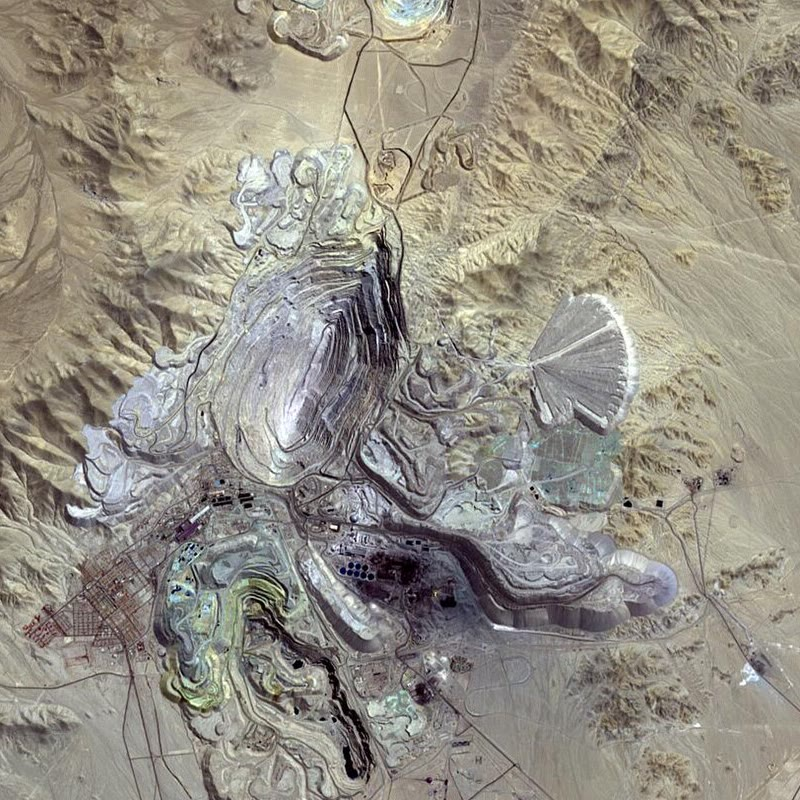
\includegraphics[width=\linewidth]{images/book1/g9-chuquicamata.jpg}
\end{minipage}\hfill
\begin{minipage}[c]{0.5\linewidth}\raggedright
{\small De kopermijn van Chuquicamata, in de Atacamawoestijn in Chili,
gezien door het instrument ASTER op een satelliet van de NASA in 2007 (het
beeld is ongeveer \qty{12}{km} breed). De ovale \omterm{def:g6:water-underground:spring}{put} in het midden, waarin
al meer dan een eeuw wordt gewerkt, is \qty{4.3}{km} lang, \qty{2.7}{km}
breed en \qty{1.1}{km} diep. NASA/METI/AIST/Japan
Space Systems en het U.S./Japan ASTER Science Team (publiek domein, via
Wikimedia Commons).}
\end{minipage}
% ledger: commons:chuquicamata, earle:chuquicamata
\label{fig:g9:earth-resources:chuquicamata}
\end{omfigure}

\paragraph{In riviergrind.} Goud roest niet en verweert nauwelijks. Als
\omterm{def:g5:water-shapes-the-land:erosion}{erosie} een goudader afbreekt, komt het goud vrij als stof, schilfers,
korrels en soms klompjes, en \omterm{def:g1:landscapes-around-us:water}{rivieren} voeren het stroomafwaarts mee. Goud
is heel dicht: ongeveer \qty{19}{g/cm^3} als het zuiver is, tegen
ongeveer \qty{2.5}{g/cm^3} voor gewoon \omterm{def:g3:stones-pebbles-sand:rock}{gesteente}. Bij \omterm{def:g5:water-shapes-the-land:flood}{overstromingen}, als
de hele bedding van \omterm{def:g3:stones-pebbles-sand:sand}{zand} en \omterm{def:g3:stones-pebbles-sand:pebble}{grind} in beweging komt, werken de zware
goudkorrels zich naar beneden en verzamelen ze zich op het \omterm{def:g3:stones-pebbles-sand:rock}{vaste gesteente}.
Geologen noemen zulke afzettingen \emph{placers}\index{placer}.
% ledger: usgs:gold-placer

\section{Steenkool, aardolie en aardgas}

Steenkool, aardolie en aardgas zijn de resten van levende wezens die
begraven werden voordat ze konden rotten. Bijna al het organische
materiaal van een dode plant of een dood dier wordt binnen weken tot
decennia weer koolstofdioxide. Alleen het deel dat van de zuurstof van de
lucht is afgesloten, op de bodem van een stilstaand moeras of van een
diepe \omterm{def:g2:water-on-earth:ocean}{zee}, kan worden begraven en miljoenen jaren bewaard blijven.
% ledger: earle:coal, earle:oil-gas

\begin{omfigure}
\begin{minipage}[c]{0.46\linewidth}\centering
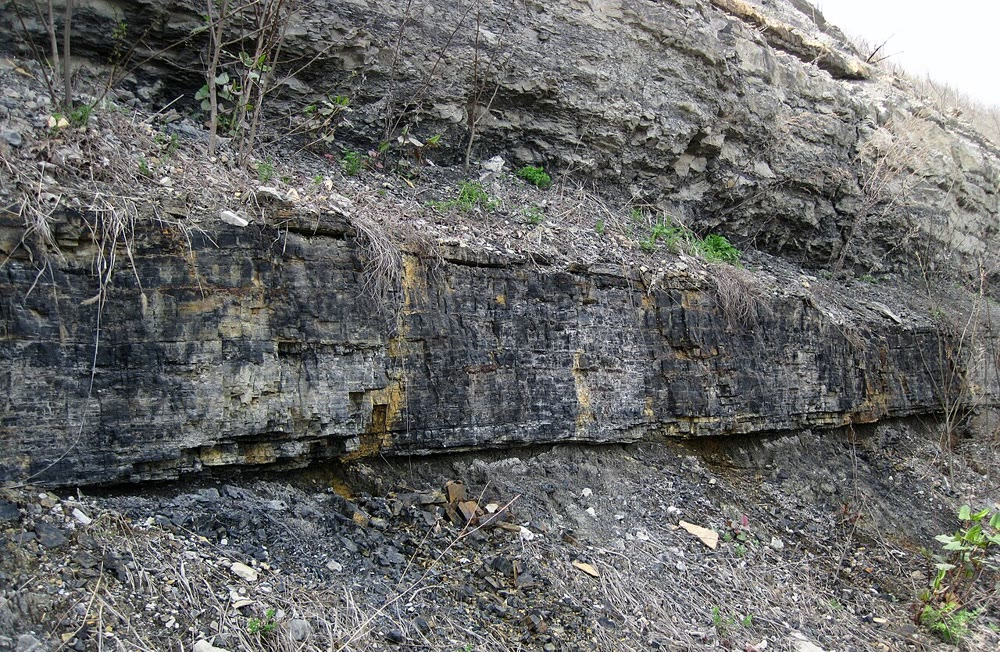
\includegraphics[width=\linewidth]{images/book1/g9-coal-seam.jpg}
\end{minipage}\hfill
\begin{minipage}[c]{0.5\linewidth}\raggedright
{\small Een steenkoollaag, de donkere laag dwars door het midden, tussen
sedimentgesteenten, langs een weg in Ohio, Verenigde Staten. De laag ligt
vlak, zoals het moeras. Foto van James St.~John (CC BY 2.0, via Wikimedia
Commons).}
\end{minipage}
% ledger: commons:meigs-coal
\label{fig:g9:earth-resources:coal-seam}
\end{omfigure}


\paragraph{Steenkool.} Steenkool begint in moerassen naast \omterm{def:g1:landscapes-around-us:water}{rivieren} en
\omterm{def:g5:water-shapes-the-land:delta}{delta's}, in warme en natte klimaten, waar planten snel groeien. Dode
stammen en bladeren vallen in stilstaand water dat weinig zuurstof bevat,
en rotten niet. Het moeras moet eeuwen tot millennia blijven bestaan om
een dikke laag op te bouwen. Op een dag verandert een \omterm{def:g1:landscapes-around-us:water}{rivier} van loop of
overstroomt ze, en bedekt ze het moeras met \omterm{def:g3:stones-pebbles-sand:sand}{zand} en modder. Naarmate er
meer \omterm{def:g7:sediments-and-fossils:sediment}{sedimenten} op komen, wordt de plantenlaag samengeperst en verwarmd,
en verandert ze in steenkool: eerst een zachte, bruine kool met ongeveer
een derde koolstof, op een paar honderd meter diepte; een harde zwarte
steenkool, met tot 86~\% koolstof, op een paar kilometer diepte. De
steenkool die nu bijvoorbeeld in de Verenigde Staten wordt gewonnen, is
meestal 100 tot 300~miljoen jaar oud.
% ledger: earle:coal, eia:coal

\begin{omfigure}
\begin{tikzpicture}[x=1cm, y=0.8cm, font=\footnotesize]
  \foreach \i/\t in {0/{(a) een moerasbos:\\ dode planten hopen\\ zich op onder\\ stil water},
                     1/{(b) begraven onder\\ zand en modder:\\ de laag wordt\\ samengeperst},
                     2/{(c) dieper en warmer\\ (honderden meters):\\ zachte bruinkool},
                     3/{(d) nog dieper\\ (kilometers):\\ harde zwarte steenkool}} {
    \begin{scope}[xshift=\i*3.35cm]
      \draw[black!40] (0,0) rectangle (2.9,4.2);
      \node[align=center, anchor=north, font=\scriptsize] at (1.45,-0.1) {\t};
    \end{scope}
  }
  % (a) swamp: water, trees, plant layer
  \fill[omSea] (0,2.6) rectangle (2.9,3.1);
  \fill[brown!60!black!70] (0,2.0) rectangle (2.9,2.6);
  \fill[omLithShale] (0,0) rectangle (2.9,2.0);
  \foreach \x in {0.5,1.4,2.3} {
    \draw[brown!50!black, line width=1.2pt] (\x,2.6) -- (\x,3.7);
    \fill[green!45!black] (\x,3.85) circle (0.3);
  }
  % (b) buried
  \begin{scope}[xshift=3.35cm]
    \fill[lith sandstone] (0,2.6) rectangle (2.9,4.0);
    \fill[brown!55!black!80] (0,2.2) rectangle (2.9,2.6);
    \fill[omLithShale] (0,0) rectangle (2.9,2.2);
    \draw[->, thick] (1.45,4.15) -- (1.45,3.45);
  \end{scope}
  % (c) lignite
  \begin{scope}[xshift=6.7cm]
    \fill[lith sandstone] (0,1.9) rectangle (2.9,4.2);
    \fill[brown!45!black] (0,1.65) rectangle (2.9,1.9);
    \fill[omLithShale] (0,0) rectangle (2.9,1.65);
  \end{scope}
  % (d) coal
  \begin{scope}[xshift=10.05cm]
    \fill[lith sandstone] (0,1.25) rectangle (2.9,4.2);
    \fill[black!85] (0,1.1) rectangle (2.9,1.25);
    \fill[omLithShale] (0,0) rectangle (2.9,1.1);
  \end{scope}
\end{tikzpicture}

{\small Van een moeras tot een steenkoollaag (een schets, niet op schaal).
Naarmate de plantenlaag dieper wegzakt, wordt ze samengeperst en verwarmd:
water en gassen ontwijken, ze wordt dunner, en haar aandeel koolstof
stijgt.}
% ledger: earle:coal, eia:coal
\label{fig:g9:earth-resources:coal}
\end{omfigure}


\paragraph{Aardolie en aardgas.} Aardolie en het meeste aardgas komen van
de piepkleine planten en dieren die in de \omterm{def:g2:water-on-earth:ocean}{zee} leven, zoals diatomeeën.
Hun resten zakken met de modder naar de zeebodem, en sommige worden
begraven voordat ze vergaan. Miljoenen jaren en kilometers \omterm{def:g7:sediments-and-fossils:sediment}{sediment} later
veranderen warmte en druk ze: onder ongeveer \qty{2}{km}, tussen ongeveer
60 en \qty{120}{\degreeCelsius}, in aardolie; bij nog hogere temperaturen
in aardgas. Aardolie en aardgas zijn lichter dan water. Ze kruipen langzaam
omhoog door de \omterm{def:g6:water-underground:porosity}{poriën} van doorlatende \omterm{def:g3:stones-pebbles-sand:rock}{gesteenten}, en veel ervan bereikt het
oppervlak en gaat verloren. Wat we vinden, is onderweg tegengehouden door
een laag \omterm{def:g6:water-underground:permeability}{ondoorlatend} \omterm{def:g3:stones-pebbles-sand:rock}{gesteente}, vaak aan de top van een opwelving, waar
het zich verzamelt: gas bovenaan, olie eronder, en water daaronder.
% ledger: eia:oil, eia:gas, earle:oil-gas

\begin{omfigure}
\begin{tikzpicture}[x=1cm, y=1cm, font=\footnotesize, >={Stealth[length=2mm]}]
  \def\fold#1{(0,#1) .. controls (3,#1+1.0) and (4.0,#1+1.6) .. (6,#1+1.6) .. controls (8.0,#1+1.6) and (9,#1+1.0) .. (12,#1)}
  % layers from the bottom up
  \fill[omLithShale!60!black!40] (0,0) -- \fold{0.9} -- (12,0) -- cycle;
  \fill[lith sandstone] \fold{0.9} -- (12,2.1) -- (12,2.1) .. controls (9,3.1) and (8.0,3.7) .. (6,3.7) .. controls (4.0,3.7) and (3,3.1) .. (0,2.1) -- cycle;
  \fill[lith shale] (0,2.1) .. controls (3,3.1) and (4.0,3.7) .. (6,3.7) .. controls (8.0,3.7) and (9,3.1) .. (12,2.1) -- (12,3.6) .. controls (9,4.6) and (8.0,5.2) .. (6,5.2) .. controls (4.0,5.2) and (3,4.6) .. (0,3.6) -- cycle;
  \fill[lith sandstone] (0,3.6) .. controls (3,4.6) and (4.0,5.2) .. (6,5.2) .. controls (8.0,5.2) and (9,4.6) .. (12,3.6) -- (12,5.6) -- (0,5.6) -- cycle;
  % gas and oil under the crest of the impermeable layer
  \fill[omWxSun!60] (4.55,3.55) .. controls (5.2,3.69) and (6.8,3.69) .. (7.45,3.55) -- (7.1,3.35) -- (4.9,3.35) -- cycle;
  \fill[black!75] (4.9,3.35) -- (7.1,3.35) -- (8.05,3.05) .. controls (7.0,3.15) and (5.0,3.15) .. (3.95,3.05) -- cycle;
  % arrows: oil creeping up through the permeable layer
  \draw[->, black, thick] (1.4,2.05) -- (2.4,2.55);
  \draw[->, black, thick] (10.6,2.05) -- (9.6,2.55);
  \draw[->, black!70] (3.0,2.65) -- (3.8,2.95);
  \draw[->, black!70] (9.0,2.65) -- (8.2,2.95);
  % labels
  \node[anchor=west, fill=white, fill opacity=0.85, text opacity=1, inner sep=1.5pt] at (0.1,0.45) {donkere modder van de oude zeebodem: hier ontstaan olie en gas};
  \node[anchor=east, fill=white, fill opacity=0.85, text opacity=1, inner sep=1.5pt] at (11.9,1.9) {doorlatende zandsteen};
  \node[anchor=east, fill=white, fill opacity=0.85, text opacity=1, inner sep=1.5pt] at (11.9,3.25) {ondoorlatende schalie};
  \node[anchor=south, fill=white, fill opacity=0.85, text opacity=1, inner sep=1.5pt] at (6,5.25) {gesteenten aan het oppervlak};
  \node[font=\scriptsize] at (6,3.48) {gas};
  \node[font=\scriptsize, text=white] at (6,3.22) {olie};
\end{tikzpicture}

{\small Aardolie en aardgas tegengehouden onder een ondoorlatende laag aan
de top van een opwelving (een schets, niet op schaal; het water dat de
rest van de zandsteen vult, is niet getekend). Onder de plooi kruipen ze
omhoog door de doorlatende zandsteen (pijlen) en verzamelen ze zich onder
de top: gas bovenaan, olie eronder.}
% ledger: earle:oil-gas
\label{fig:g9:earth-resources:oil}
\end{omfigure}

\section{Water uit de grond}

Ook \omterm{def:g6:water-underground:groundwater}{grondwater} is een grondstof uit de Aarde, de grondstof die we elke dag
gebruiken. Anders dan een metaal of steenkool wordt het aangevuld: \omterm{def:g4:clouds-rain-snow:precipitation}{regen}
vult de watervoerende lagen weer aan. Maar dat gebeurt langzaam, en maar
zo snel als de \omterm{def:g4:clouds-rain-snow:precipitation}{regen} in de grond trekt. Bij een \omterm{def:g6:water-underground:aquifer}{watervoerende laag} die
sneller wordt leeggepompt dan ze wordt aangevuld, daalt de
\omterm{def:g6:water-underground:water-table}{grondwaterspiegel}, en vallen putten droog (\cref{ch:g6:water-underground}).
\omterm{def:g6:water-underground:groundwater}{Grondwater} is alleen een hernieuwbare grondstof zolang het niet sneller
wordt opgepompt dan het wordt aangevuld.
% ledger: wss:aquifer

\section{Zand en grind}

Het vaste materiaal dat mensen in de grootste hoeveelheden uit de grond
halen, is geen steenkool en geen metaalerts: het is \omterm{def:g3:stones-pebbles-sand:sand}{zand} en \omterm{def:g3:stones-pebbles-sand:pebble}{grind}.
% ledger: tos:sand

\begin{definition}[Toeslagmateriaal]\label{def:g9:earth-resources:aggregate}
\emph{Toeslagmaterialen}\index{toeslagmateriaal} zijn het \omterm{def:g3:stones-pebbles-sand:sand}{zand}, het \omterm{def:g3:stones-pebbles-sand:pebble}{grind}
en de steenslag die in de bouw worden gebruikt: in beton, onder wegen en
spoorlijnen, en om de grond op te hogen.
\end{definition}
% ledger: usgs:aggregate, tos:sand

Het meeste \omterm{def:g3:stones-pebbles-sand:sand}{zand} gaat in beton, een mengsel van \omterm{def:g3:stones-pebbles-sand:sand}{zand}, \omterm{def:g3:stones-pebbles-sand:pebble}{grind}, water en
cement. In 2019 had de wereld ongeveer 50~miljard ton \omterm{def:g3:stones-pebbles-sand:sand}{zand} en \omterm{def:g3:stones-pebbles-sand:pebble}{grind} per
jaar nodig, dat is $5 \times 10^{10}$ ton, of ongeveer \qty{18}{kg} per
persoon op Aarde, elke dag. \omterm{def:g3:stones-pebbles-sand:sand}{Zand} en \omterm{def:g3:stones-pebbles-sand:pebble}{grind} worden gewonnen uit groeven op
het land, uit rivierbeddingen en, steeds meer, van de zeebodem. Wordt het
uit een \omterm{def:g1:landscapes-around-us:water}{rivier} gehaald, dan bereikt er minder \omterm{def:g3:stones-pebbles-sand:sand}{zand} de \omterm{def:g1:landscapes-around-us:water}{kust}, en slijten
stranden stroomafwaarts weg.
% ledger: tos:sand

\begin{omfigure}
\begin{minipage}[c]{0.46\linewidth}\centering
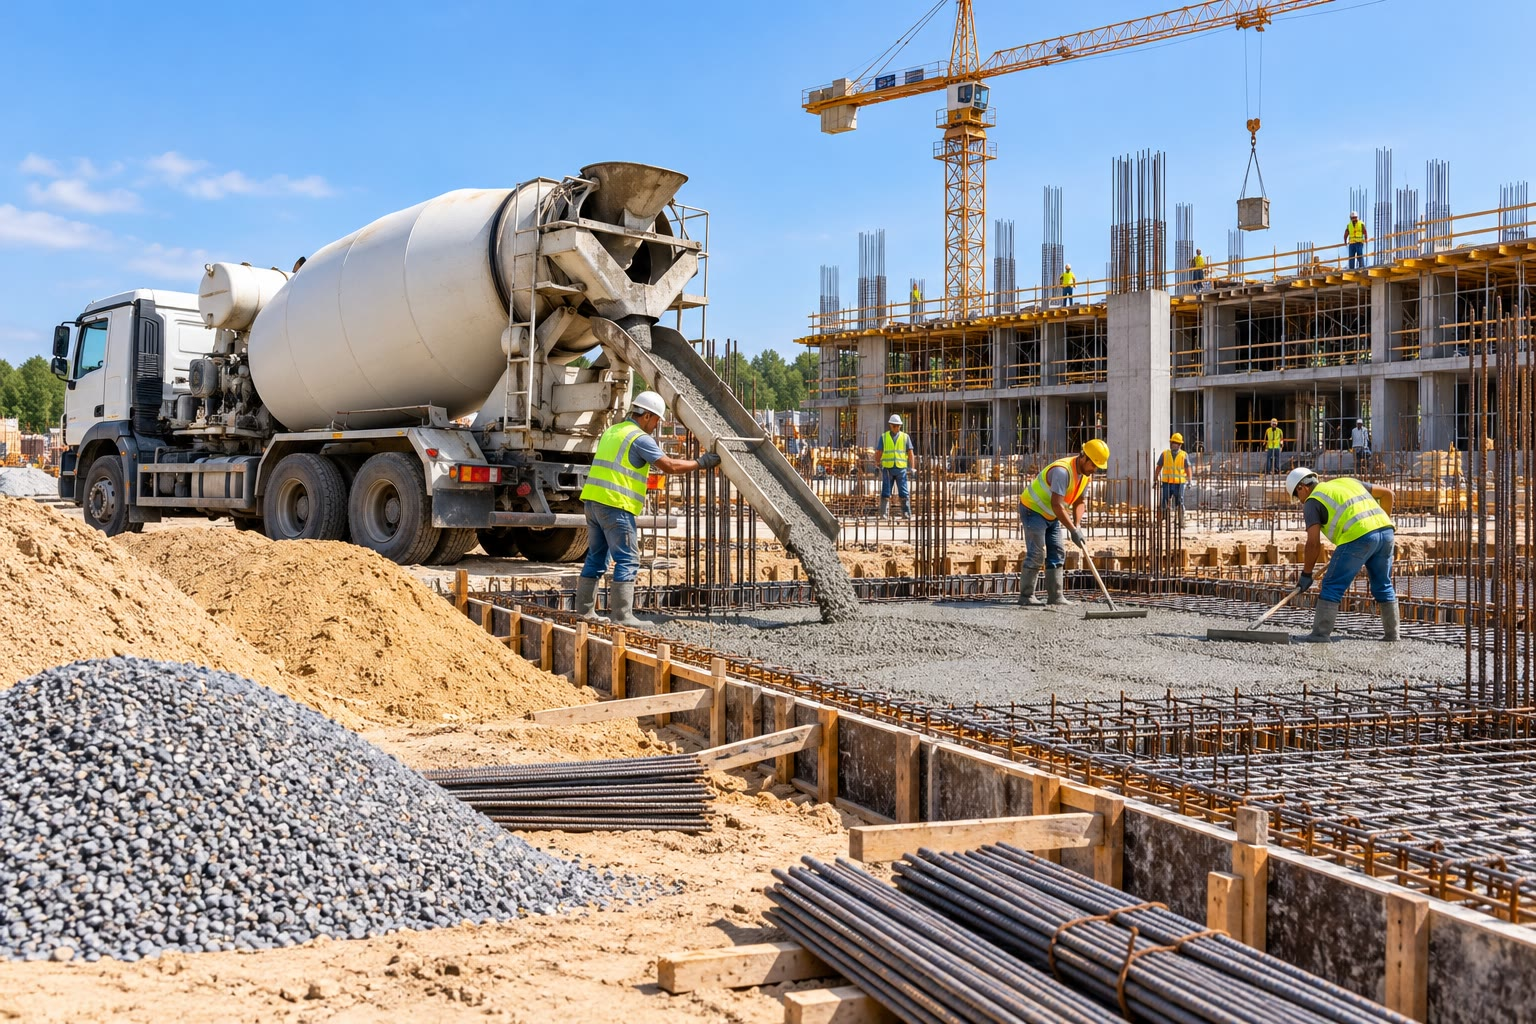
\includegraphics[width=\linewidth]{images/book1/ai/g9-building-site.jpg}
\end{minipage}\hfill
\begin{minipage}[c]{0.5\linewidth}\raggedright
{\small \omterm{def:g9:earth-resources:aggregate}{Toeslagmaterialen} aan het werk: hopen \omterm{def:g3:stones-pebbles-sand:sand}{zand} en \omterm{def:g3:stones-pebbles-sand:pebble}{grind} naast een
betonmixer die de vloer van een nieuw gebouw stort (door AI gegenereerde
illustratie van een algemene scène).}
\end{minipage}
\label{fig:g9:earth-resources:building-site}
\end{omfigure}

\section{Hernieuwbaar of eindig?}

Een grondstof die de natuur binnen een mensenleven aanvult, zoals het
water van een \omterm{def:g6:water-underground:aquifer}{watervoerende laag} die niet wordt overbepompt, kan voor
altijd worden gebruikt. Een \omterm{def:g9:earth-resources:ore-deposit}{ertsafzetting}, een steenkoollaag of een
olieveld heeft miljoenen jaren nodig gehad om te ontstaan. Wij gebruiken
het in een paar decennia op: op onze tijdschaal wordt het helemaal niet
aangevuld.
% ledger: eia:coal, earle:coal

\begin{omfigure}
\begin{tikzpicture}
\begin{axis}[xmode=log, width=12.5cm, height=4.6cm, xmin=10, xmax=1e9, ymin=0.4, ymax=4.6,
  ytick=\empty, xlabel={jaren (logaritmische schaal)}, label style={font=\small},
  xtick={10,100,1000,1e4,1e5,1e6,1e7,1e8,1e9},
  xticklabels={$10$,$10^2$,$10^3$,$10^4$,$10^5$,$10^6$,$10^7$,$10^8$,$10^9$},
  tick label style={font=\footnotesize}, xmajorgrids, grid style={black!12}, clip=false]
\addplot[only marks, mark=|, mark size=4pt, line width=4pt, omWarm,
  error bars/.cd, x dir=plus, x explicit, error bar style={line width=4pt, omWarm}, error mark=none]
  table[x=lo_yr, y=y, x error expr=\thisrow{hi_yr}-\thisrow{lo_yr}] {figdata/out/grade-9-concentration-times.dat};
\node[anchor=west, font=\footnotesize, fill=white, inner sep=1pt] at (axis cs:1500,4) {een moeras bouwt een dikke laag planten op};
\node[anchor=east, font=\footnotesize, fill=white, inner sep=1pt] at (axis cs:6e7,3) {ouderdom van steenkool uit de Verenigde Staten};
\node[anchor=west, font=\footnotesize, fill=white, inner sep=1pt] at (axis cs:150,2) {Chuquicamata, tot nu toe ontgonnen (meer dan een eeuw)};
\node[anchor=west, font=\footnotesize, fill=white, inner sep=1pt] at (axis cs:65,1) {wereldreserves koper bij het mijnbouwtempo van 2024};
\end{axis}
\end{tikzpicture}

{\small Tijden van ontstaan en tijden van gebruik, op een schaal waarin
elke stap tien keer de vorige is. De steenkool is ongeveer een miljoen
keer ouder dan de tijd die een mijn nodig heeft om een afzetting leeg te
halen.}
% ledger: earle:coal, eia:coal, earle:chuquicamata, usgs:mcs-copper (figdata/grade-9/concentration.py, part times)
\label{fig:g9:earth-resources:times}
\end{omfigure}

Hoe lang gaat een grondstof mee? Geologen tellen alleen wat bekend is en
kan worden gewonnen.

\begin{definition}[Reserve]\label{def:g9:earth-resources:reserve}
De \emph{reserve}\index{reserve} van een minerale grondstof is het deel van
de bekende afzettingen dat met winst kan worden gewonnen, met de
technieken en de prijzen van dat moment.
\end{definition}
% ledger: usgs:mcs-reserves

Een \omterm{def:g9:earth-resources:reserve}{reserve} is niet alles wat er in de grond zit. Ze groeit als er nieuwe
afzettingen worden gevonden, als de technieken verbeteren of als de prijzen
stijgen, en ze krimpt naarmate de afzettingen worden ontgonnen. In 1970
werden de koperreserves van de wereld geschat op 280~miljoen ton. Sindsdien
is er ongeveer 700~miljoen ton koper gewonnen, tweeënhalf keer die
\omterm{def:g9:earth-resources:reserve}{reserve}, en toch werden de \omterm{def:g9:earth-resources:reserve}{reserves} van 2024 geschat op 980~miljoen ton.
% ledger: usgs:mcs-reserves

\begin{dated}{2025}
In 2024 produceerden de mijnen van de wereld ongeveer 23~miljoen ton
koper. In dat tempo zouden de \omterm{def:g9:earth-resources:reserve}{reserves} van 980~miljoen ton $980 \div 23
\approx 43$ jaar meegaan. Zo'n getal is geen datum waarop het koper op is:
het is een maat voor het koper dat bekend is en dat het nu waard is om te
winnen.
\end{dated}
% ledger: usgs:mcs-copper (figdata/grade-9/concentration.py: 42.6 years)

Een metaal wordt, anders dan steenkool of aardolie, niet vernietigd als het
wordt gebruikt: het recyclen van materialen, dat je in de scheikundeboeken
tegenkomt, geeft het terug. Het koper van een oude kabel, van een
gesloopte motor of van de restjes van een fabriek kan opnieuw worden
gesmolten en geraffineerd. In de Verenigde Staten maakte in 2024 koper dat
uit schroot was teruggewonnen ongeveer \qty{35}{\%} uit van al het
gebruikte koper.
% ledger: usgs:mcs-copper-scrap

\begin{omfigure}
\begin{tikzpicture}[font=\footnotesize, node distance=1.2cm,
  box/.style={draw=black!60, fill=black!4, rounded corners=2pt, align=center, minimum height=0.9cm, inner sep=3pt},
  flow/.style={-{Stealth[length=2.2mm]}, line width=0.9pt, black!70}]
  \node[box, fill=omWarm!12] (ore) at (0,0) {ertsafzetting\\(gesteente met\\\qty{0.5}{\%} koper)};
  \node[box] (metal) at (4.2,0) {kopermetaal};
  \node[box] (things) at (8.2,0) {kabels, buizen,\\motoren};
  \node[box, fill=blue!8] (scrap) at (6.2,-2.1) {schroot};
  \node[box, fill=black!12] (waste) at (0,-2.1) {overgebleven\\vermalen gesteente};
  \draw[flow] (ore) -- node[above] {winnen,} node[below] {verrijken} (metal);
  \draw[flow] (metal) -- node[above] {maken} (things);
  \draw[flow] (things) |- node[pos=0.25, right] {weggegooid} (scrap);
  \draw[flow] (scrap) -| node[pos=0.75, left] {smelten, raffineren} (metal);
  \draw[flow] (ore) -- (waste);
\end{tikzpicture}

{\small Twee wegen naar kopermetaal: uit een erts, via tonnen afgegraven
en vermalen \omterm{def:g3:stones-pebbles-sand:rock}{gesteente}, of uit schroot, dat opnieuw wordt gesmolten en
geraffineerd.}
\end{omfigure}

\begin{example}[Het gesteente dat recyclen uitspaart]\label{ex:g9:earth-resources:recycling}
Een erts met \qty{0.5}{\%} koper bevat \qty{5}{kg} koper per ton \omterm{def:g3:stones-pebbles-sand:rock}{gesteente}.
Om één ton koper te maken, moet er ongeveer $1000 \div 5 = 200$ ton erts
worden afgegraven, vermalen en behandeld, en bijna alles daarvan eindigt
als afvalgesteente. Elke ton koper die uit schroot wordt gemaakt, laat die
200 ton \omterm{def:g3:stones-pebbles-sand:rock}{gesteente} in de grond --- en de afzetting gaat langer mee.
% ledger: perkins:ore-grades (computed)
\end{example}


\section{Oefeningen}

\begin{exercise}[$\star$]\label{exo:g9:earth-resources:1}
Vul het juiste woord in (\omterm{def:g9:earth-resources:ore-deposit}{ertsafzetting}, \omterm{def:g9:earth-resources:ore-deposit}{concentratiefactor},
\omterm{def:g9:earth-resources:aggregate}{toeslagmateriaal}, \omterm{def:g9:earth-resources:reserve}{reserve}). (a) \omterm{def:g3:stones-pebbles-sand:sand}{Zand} dat in beton wordt gebruikt, is een
\ldots\ (b) Het deel van het bekende koper dat nu met winst kan worden
gewonnen, is de \ldots\ aan koper. (c) Een \omterm{def:g3:stones-pebbles-sand:rock}{gesteente} waarin een metaal
rijk genoeg is om te worden gewonnen, is een \ldots\ (d) Het aantal keer
dat een metaal is geconcentreerd, is zijn \ldots
\end{exercise}

\begin{exercise}[$\star$]\label{exo:g9:earth-resources:2}
% ledger: earle:magmatic, usgs:gold-lode, usgs:gold-placer
Welke manier om een metaal te concentreren beschrijft elke zin: in het
\omterm{def:g7:volcanoes:magma}{magma}, in spleten uit heet water, of in riviergrind? (a) Goudklompjes
liggen op het \omterm{def:g3:stones-pebbles-sand:rock}{vaste gesteente} onder het \omterm{def:g3:stones-pebbles-sand:pebble}{grind} van een beek. (b) Heet water
vult een spleet met kwarts en goud. (c) Een laag zware nikkelmineralen
ligt op de bodem van een oude magmamassa. (d) Goud wordt door \omterm{def:g5:water-shapes-the-land:erosion}{erosie} uit
een ader vrijgemaakt.
\end{exercise}

\begin{exercise}[$\star$]\label{exo:g9:earth-resources:3}
% ledger: earle:coal, eia:coal
Zet deze stappen in de juiste volgorde: (a) de plantenlaag wordt onder
rivierzand begraven; (b) er groeien bomen in een moeras; (c) op
kilometers diepte ontstaat een harde zwarte steenkool; (d) dode planten
stapelen zich op onder stil water; (e) er ontstaat een zachte bruinkool.
\end{exercise}

\begin{exercise}[$\star$]\label{exo:g9:earth-resources:4}
Is elke grondstof op de schaal van een mensenleven hernieuwbaar of niet?
Leg uit in één zin. (a) Steenkool. (b) Het water van een \omterm{def:g6:water-underground:aquifer}{watervoerende laag}
die minder wordt leeggepompt dan de \omterm{def:g4:clouds-rain-snow:precipitation}{regen} aanvult. (c) Kopererts.
(d) Dezelfde \omterm{def:g6:water-underground:aquifer}{watervoerende laag}, twee keer zo snel leeggepompt als ze
wordt aangevuld.
\end{exercise}

\begin{exercise}[$\star\star$]\label{exo:g9:earth-resources:5}
% ledger: perkins:ore-grades
Bereken de \omterm{def:g9:earth-resources:ore-deposit}{concentratiefactor} en schrijf hem dan afgerond als macht van
tien: (a) zink, \qty{0.007}{\%} in de korst, erts vanaf \qty{4}{\%};
(b) tin, \qty{0.0002}{\%} in de korst, erts vanaf \qty{0.5}{\%};
(c) ijzer, \qty{5.6}{\%} in de korst, erts vanaf \qty{20}{\%}. (d) Waarom
hoeft ijzer zo weinig te worden geconcentreerd?
\end{exercise}

\begin{exercise}[$\star\star$]\label{exo:g9:earth-resources:6}
% ledger: usgs:gold-placer
Zuiver goud heeft een dichtheid van ongeveer \qty{19.3}{g/cm^3}; gewoon
\omterm{def:g3:stones-pebbles-sand:rock}{gesteente} ongeveer \qty{2.5}{g/cm^3}. (a) Hoeveel keer dichter is goud?
(b) Wat is de massa van een goudkorrel van \qty{0.01}{cm^3}, en van een
gesteentekorrel van dezelfde grootte? (c) Leg uit waarom het goud bij een
\omterm{def:g5:water-shapes-the-land:flood}{overstroming} onderaan het \omterm{def:g3:stones-pebbles-sand:pebble}{grind} terechtkomt, op het \omterm{def:g3:stones-pebbles-sand:rock}{vaste gesteente}.
\end{exercise}

\begin{exercise}[$\star\star$]\label{exo:g9:earth-resources:7}
% ledger: perkins:ore-grades, earle:ore-grades (figdata/grade-9/concentration.py)
Gebruik de grafiek van de \omterm{def:g9:earth-resources:ore-deposit}{concentratiefactoren}. (a) Welke metalen hebben
een factor van meer dan $10^3$ nodig? (b) Tussen welke machten van tien
ligt koper? (c) Hoeveel keer meer moet chroom worden geconcentreerd dan
aluminium? (d) Van welk van de zeven metalen verwacht je dat het op de
minste plaatsen wordt gewonnen? Leg uit.
\end{exercise}

\begin{exercise}[$\star\star$]\label{exo:g9:earth-resources:8}
% ledger: tos:sand
De wereld heeft ongeveer \qty{18}{kg} \omterm{def:g3:stones-pebbles-sand:sand}{zand} en \omterm{def:g3:stones-pebbles-sand:pebble}{grind} per persoon per dag
nodig. (a) Hoeveel is dat per persoon in één jaar, in ton? (b) Schrijf 50
miljard ton in de wetenschappelijke notatie. (c) Een vrachtwagen vervoert
\qty{25}{t}. Na hoeveel dagen vult het aandeel van één persoon hem?
(d) Waarom kan het weghalen van \omterm{def:g3:stones-pebbles-sand:sand}{zand} uit een \omterm{def:g1:landscapes-around-us:water}{rivier} een strand
stroomafwaarts doen krimpen?
\end{exercise}

\begin{exercise}[$\star\star$]\label{exo:g9:earth-resources:9}
% ledger: earle:oil-gas, eia:oil
(a) Van welke levende wezens komen de meeste aardolie en het meeste
aardgas? (b) Bij welke temperaturen ontstaat aardolie onder ongeveer
\qty{2}{km}? (c) Waarom bewegen aardolie en aardgas omhoog door de
\omterm{def:g3:stones-pebbles-sand:rock}{gesteenten}? (d) Welk soort \omterm{def:g3:stones-pebbles-sand:rock}{gesteente} houdt ze tegen, en waar verzamelen ze
zich?
\end{exercise}

\begin{exercise}[$\star\star$]\label{exo:g9:earth-resources:10}
% ledger: earle:chuquicamata
De mijn van Chuquicamata heeft in meer dan 100 jaar meer dan 29~miljoen
ton koper geproduceerd. (a) Schrijf 29~miljoen ton in de
wetenschappelijke notatie. (b) Wat is ruwweg de gemiddelde productie per
jaar? (c) Als het erts \qty{1}{\%} koper bevatte, hoeveel ton erts is er
dan afgegraven om 29~miljoen ton koper te krijgen? Gebruik de
wetenschappelijke notatie. (d) Waarom moet een mijn met zo'n arm erts zo
groot zijn?
\end{exercise}

\begin{exercise}[$\star\star\star$]\label{exo:g9:earth-resources:11}
% ledger: usgs:mcs-reserves, usgs:mcs-copper
In 1970 werden de koperreserves van de wereld geschat op 280~miljoen ton.
Van 1970 tot 2024 werd er ongeveer 697~miljoen ton gewonnen, en de
\omterm{def:g9:earth-resources:reserve}{reserves} van 2024 waren 980~miljoen ton, met 23~miljoen ton gewonnen in
2024. (a) Als de \omterm{def:g9:earth-resources:reserve}{reserve} van 1970 al het koper was geweest dat er was,
wanneer zou het dan op zijn geweest? Vergelijk met wat er is gewonnen.
(b) Hoeveel keer groter is de \omterm{def:g9:earth-resources:reserve}{reserve} van 2024 dan die van 1970?
(c) Bereken hoeveel jaar de \omterm{def:g9:earth-resources:reserve}{reserve} van 2024 zou meegaan in het tempo van
2024. (d) Geef twee redenen waarom een \omterm{def:g9:earth-resources:reserve}{reserve} kan groeien terwijl ze
wordt ontgonnen.
\end{exercise}

\begin{exercise}[$\star\star\star$]\label{exo:g9:earth-resources:12}
% ledger: earle:coal, eia:coal
Een steenkoollaag is $3 \times 10^8$ jaar oud. Het moeras ervan bestond
$2 \times 10^3$ jaar, en de laag wordt in 50 jaar leeggehaald.
(a) Schrijf 50 jaar in de wetenschappelijke notatie. (b) Hoeveel keer
langer dan de mijnbouw bestond het moeras? (c) Hoeveel keer ouder dan de
duur van de mijnbouw is de laag? (d) Leg met deze getallen uit waarom
steenkool een niet-hernieuwbare grondstof wordt genoemd.
\end{exercise}

\section{Probleem: Beton voor een nieuwe stad}

\begin{problem}[{Weekendprobleem --- een nieuwe stad wordt gebouwd met het
zand van een plaatselijke groeve; het eindantwoord is het aantal jaren
dat de zandreserve van de groeve zou meegaan}]
\label{pb:g9:earth-resources:1}
% ledger: usgs:aggregate (about 100 and 300 t per home), tos:sand (figdata/grade-9/concentration.py, part problem: exercise data)
Een nieuwe stad van \num{2000} woningen moet in tien jaar worden gebouwd,
dicht bij een oude zandgroeve die is gegraven in het \omterm{def:g3:stones-pebbles-sand:pebble}{grind} van een
rivierterras. Met haar aandeel in de straten, de scholen en de winkels
heeft elke woning ongeveer \qty{300}{t} \omterm{def:g9:earth-resources:aggregate}{toeslagmaterialen} nodig, waarvan
\qty{40}{\%} \omterm{def:g3:stones-pebbles-sand:sand}{zand}. De zandlaag van de groeve is \qty{1.2}{km} lang,
\qty{500}{m} breed en \qty{5}{m} dik; één kubieke meter van haar \omterm{def:g3:stones-pebbles-sand:sand}{zand} heeft
een massa van \qty{1.6}{t}. De groeve verkoopt ook \num{136000} ton \omterm{def:g3:stones-pebbles-sand:sand}{zand}
per jaar aan de rest van de regio.

\noindent\textbf{Deel I --- Hoeveel zand?}\par\nopagebreak
\begin{enumerate}[beginpenalty=10000]
  \item Een eengezinshuis alleen heeft ongeveer \qty{100}{t}
        \omterm{def:g9:earth-resources:aggregate}{toeslagmaterialen} nodig. Schrijf deze massa in kilogram, in de
        wetenschappelijke notatie.
  \item Hoeveel ton \omterm{def:g9:earth-resources:aggregate}{toeslagmaterialen} heeft de hele stad nodig?
  \item Hoeveel ton is dat per jaar, over de tien jaar?
  \item Hoeveel ton \omterm{def:g3:stones-pebbles-sand:sand}{zand} per jaar heeft de stad nodig?
\end{enumerate}

\noindent\textbf{Deel II --- De reserve.}\par\nopagebreak
\begin{enumerate}[resume, beginpenalty=10000]
  \item Bereken het volume van de zandlaag, in kubieke meter, in de
        wetenschappelijke notatie.
  \item Een derde van de laag ligt onder een dorp en een weg en wordt niet
        afgegraven. Welk volume kan worden gewonnen?
  \item Wat is de massa van deze \omterm{def:g9:earth-resources:reserve}{reserve}, in ton?
  \item Hoeveel ton \omterm{def:g3:stones-pebbles-sand:sand}{zand} zal de groeve elk jaar verkopen, aan de stad en
        aan de regio samen?
\end{enumerate}

\noindent\textbf{Deel III --- Hernieuwbaar of niet?}\par\nopagebreak
\begin{enumerate}[resume, beginpenalty=10000]
  \item Elk jaar voert de \omterm{def:g1:landscapes-around-us:water}{rivier} ongeveer \num{2000} ton nieuw \omterm{def:g3:stones-pebbles-sand:sand}{zand} naar het
        gebied aan. Hoeveel keer meer \omterm{def:g3:stones-pebbles-sand:sand}{zand} verkoopt de groeve?
  \item Is dit \omterm{def:g3:stones-pebbles-sand:sand}{zand} op de schaal van het leven van de stad een
        hernieuwbare grondstof? Leg uit.
  \item Als de stad een kwart van haar \omterm{def:g3:stones-pebbles-sand:sand}{zand} verving door vermalen oud
        beton, hoeveel ton \omterm{def:g3:stones-pebbles-sand:sand}{zand} zou ze dan elk jaar uitsparen?
  \item Hoeveel jaar zou de zandreserve van de groeve zonder die recycling
        meegaan?
\end{enumerate}
\end{problem}
